\RequirePackage[hyphens]{url}
\documentclass{sig-alternate-05-2015}
\usepackage{graphicx}
\usepackage[marginal]{footmisc}
\usepackage{cite}
\usepackage{hyperref}
\usepackage{color}
\usepackage{listings}
\usepackage{cprotect}
\usepackage{multirow}
%\usepackage{tabularx}


\definecolor{mygreen}{rgb}{0,0.6,0}
\definecolor{mygray}{rgb}{0.5,0.5,0.5}
\definecolor{mymauve}{rgb}{0.58,0,0.82}

\lstset{
  numbers=left,
  showstringspaces=false,
  xleftmargin=0em,
  framexleftmargin=0em,
  frame=single,
  commentstyle=\it,
  basicstyle=\ttfamily\scriptsize,
  commentstyle=\color{mygreen},
  numberstyle=\tiny\color{mygray},
  stringstyle=\color{mymauve},
  keywordstyle=\color{blue}
}

\lstdefinestyle{myCompactStyle}{
  xleftmargin=0em,
  framexleftmargin=0em,
  numbers=none,
  stepnumber=1,
  tabsize=4,
  basicstyle=\ttfamily,
  keywordstyle=\bfseries,
  showspaces=false,
  showstringspaces=false
}

\lstdefinelanguage{scala}{
  morekeywords={abstract,case,catch,class,def,%
    do,else,extends,false,final,finally,%
    for,if,implicit,import,match,mixin,%
    new,null,object,override,package,%
    private,protected,requires,return,sealed,%
    super,this,throw,trait,true,try,%
    type,val,var,while,with,yield},
  otherkeywords={=>,<-,<\%,<:,>:,\#,@},
  sensitive=true,
  morecomment=[l]{//},
  morecomment=[n]{/*}{*/},
  morestring=[b]",
  morestring=[b]',
  morestring=[b]"""
}


\newtheorem{rem}{Remark}
\def\SS{{\textit{LSearcher}}}

\newcommand{\todo}[1]{{\footnotesize \textcolor{red}{$\ll$\textsf{TODO #1}$\gg$}}}%

\begin{document}

\title{LSearcher: A DBLP Search Engine Based on Lucene}


\numberofauthors{4}
\author{
\alignauthor Chen Hongxu, {SCSE}\\
       \email{hchen017@e.ntu.edu.sg}
% 2nd. author
\alignauthor
Feng Ruitao, {SCSE}\\
       \email{feng0082@e.ntu.edu.sg}
%% 3rd. author
\alignauthor
Zhou Yuan, {SCSE}\\
       \email{yzhou027@e.ntu.edu.sg}
\and  % use '\and' if you need 'another row' of author names
%% 4th. author
\alignauthor Zhu Jingyang, {WKW}\\
       \email{W150016@e.ntu.edu.sg}
}

\maketitle

\begin{abstract}
A search engine is an information retrieval system designed to help the users to retrieve stored information. In this study, we implement a search engine, {\SS}, aiming to retrieve publication information in DBLP.
{\SS} focuses on searching for articles published in journals, conferences, and workshop proceedings. The input queries can be authors, paper titles, publication venues, and$/$or their combinations. The returned results of each query are top-$N$ relevant records.
It is further applied to two applications: (1) searches for the top-$N$ popular research topics in a year, possibly constrained to other attribute preconditions such publication venues or authors; and (2) searches for the top-$N$ publication venues that are most similar with a given one.
\end{abstract}


\keywords{Information retrieval; Search engine; DBLP; Lucene}

\section{Introduction}

Information Retrieval (IR) tries to find material (usually documents) of an unstructured nature (usually text) that satisfies an information need from within large collections~\cite{MRS08}. A search engine provides an interface to a group of items that enables users to specify criteria about a given information need and have the engine find the material~\cite{search-engine}. The search results are a list of relevant items.
Search engines help humans to minimize the time to find information and the amount of information to be consulted.
There are many kinds of search engines aiming at different domains, such as web search engine, visual search engine, enterprise search engine, desktop search engine, and so on \cite{list-of-engine}.

In this study, we focus on the retrieval of the publication records in DBLP (\textbf{D}igital \textbf{B}ibliography \& \textbf{L}ibrary \textbf{P}roject).
DBLP is a computer science bibliography which provides open bibliographic information on major computer science publications. It records papers from many resources, such as journals, magazines, conferences and workshops, informal publications, and so on. For simplicity, in our project, we only consider articles and inproceedings. The raw DBLP data is in a single daily-updated XML file\footnote{\url{http://dblp.uni-trier.de/xml/}}. The xml file used in our experiments was retrieved on 22 February, 2016.

A search engine called {\SS} is developed in this study. It can search for the publication records based on user queries. Besides, users can also search for the top-$N$ topics in a single year or top-$N$ publication venues in a specific year that are similar with the given one.

The objective of this work is to practice and be familiar with (1) the basic knowledge of IR, such as term weighting schemes (e.g., IT-IDF based measures), indexing process, ranking mechanisms, and evaluation for a search engine, and (2) the details for the development of a basic search engine with the help of third-party libraries. 

The rest of this paper is organized as follows. Section \ref{sec:overview} gives an overview of the main processes for a search engine; section~\ref{sec:impl-overview} gives a blueprint of the implementations; section~\ref{sec:extraction} talks about the data extraction from xml file; section \ref{sec:proj1} shows the indexing and searching implementation details as well as the evaluations; section \ref{sec:proj2} talks about the two IR applications; Section \ref{sec:discuss} contains discussions on the implementation method; and section \ref{sec:conclusion} concludes our work.

\section{Overview of a Search Engine}\label{sec:overview}

In this section, we give a brief description of the workflow and evaluation of a search engine.
A search engine typically consists of two processes, i.e., indexing process and matching process~\cite{V99}.
Indexing is the process of selecting terms to represent a text.
Matching is the process of applying a retrieval model to feed back relevant documents.
Fig.~\ref{fig:frame} shows the general workflow of an engine to search for the information need in a collection of material.
\begin{figure}
  \centering
  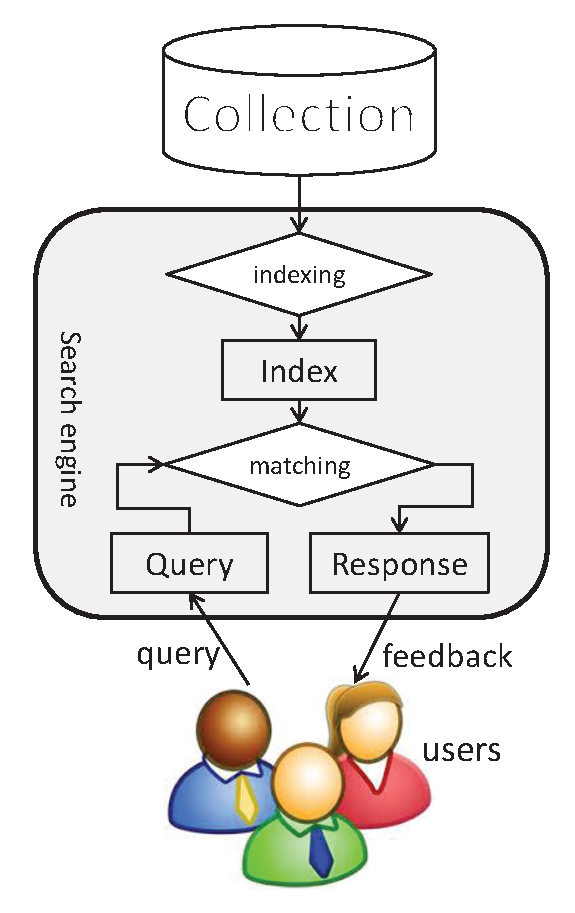
\includegraphics[width=.5\columnwidth]{frame1}
  \caption{The framework of a search engine.}\label{fig:frame}
\end{figure}

\subsection{Indexing}

In order to be searchable, the dataset should firstly be indexed and stored.
A general indexing process usually contains following steps.
\begin{enumerate}
  \item \textbf{Tokenization}. Break apart the components (e.g., words) of a document.
  \item \textbf{Removal of stop words}. Remove frequently used words such as prepositions and pronouns.
  \item \textbf{Stemming}. Conflate related word forms to a common stem by removing suffixes.
  \item \textbf{Index construction}. Build an appropriate index for the system to further search.
\end{enumerate}

The main step is to build an appropriate search index. It can provide the results for queries.
Without a search engine index, the search engine would take considerable
amounts of time and effort each time a search query is initiated.
There are two main parts in a search engine index, i.e., design factors and data structures.
The design factors of a search engine index outline the architecture of the index and decide how the index actually works, such as merge factors, index size, storage techniques, and so on.
The data structures of a search engine index can be forward index, inverted index, document-term matrix, and so on.

\subsection{Retrieval models}

After obtaining the search engine index, a proper retrieval model is applied to find the relevant documents and their rankings. There are many retrieval models available.

%The simplest IR model is the Boolean model. In this model, the index is a document-term matrix. The queries are represented as Boolean combinations of terms, and the set of documents that satisfied the Boolean expression was retrieved in response to the query. We only need to consider whether a term is in a document or not, without counting the frequency of each term in a document.  Moreover, we cannot rank the returned results.

The vector space model is a commonly used retrieval model.
It casts queries and documents as finite dimensional vectors, where each element is the weight of a term in a document computed using numerous variations of TF-IDF. To compute a score between a document and a query, the model needs to measure the similarity between the query and document vectors, such as using cosine function. Thus, the main task is to construct a proper term weight scheme.
A basic TF-IDF weighting scheme can be described as follows~\cite{MRS08}.
Suppose $C$ is a document collection with $N$ documents, $d$ is a document, and $t$ is a term.
The term frequency (TF) of $t$ in $d$, denoted as $tf_{t,d}$, is defined as the number of occurrences of term $t$ in document $d$.
The document frequency of $t$, denoted as $df_t$, is the number of documents that contain $t$ in the collection $C$, and the inverse document frequency (IDF) is defined as $idf_t=\frac{N}{df_t}$.
Thus, the final term weighting of $t$ in $d$ can be described as:
\begin{equation}
	  w_{t,d}=\left\{
  \begin{array}{ll}
    (1+\log_{10}tf_{t,d})\times \log_{10}\frac{N}{df_t}, & tf_{t,d}>0 \wedge df_{t}>0\\
    0, & tf_{t,d}\cdot df_{t}=0
  \end{array}\right.
\end{equation}
The final score for document $d$ corresponding to query $q$ can be measured by the summation of the weights of matched terms (Eq. \ref{eq:sum}),  or the cosine similarity (Eq. \ref{eq:cos}).
\begin{equation}\label{eq:sum}
  score(q,d)=\sum_{t\in q\cap d}w_{t,d}
\end{equation}
\begin{equation}\label{eq:cos}
  cos(\vec{q},\vec{d})=\frac{\vec{q}\cdot \vec{d}}{\|\vec{q}\|\|\vec{d}\|}=\frac{\sum_{i=1}^{|V|} q_id_i}{\sqrt{\sum_{i=1}^{|V|} q_i^2}\sqrt{\sum_{i=1}^{|V|} d_i^2}}
\end{equation}
where $\vec{q}$ and $\vec{d}$ are the weighted vectors whose elements are the weights of the collection's terms in $q$ and $d$, respectively; $q_i$ and $d_i$ are the term weight of term $i$ in $q$ and $d$, respectively; and $|V|$ is the number of terms in collection $C$.


%Note that in \emph{Lucene}, the scoring function is defined as
%\begin{equation}\label{lucenescore}
%  score(q,d)=coord(q,d)\cdot queryNorm(q) \cdot (\sum_{t\in q} (tfw_{t,d} \cdot idf_t^2 \cdot t.))
%\end{equation}
%the TF weight of a term $t$ in document $d$, denoted as $tfw_{t,d}$, is defined as $tfw_{t,d}=\sqrt{tf_{t,d}}$, and the IDF weight of a term $t$ in document $d$ is defined as $idfw_t=1+\frac{N}{df_{t}+1}$.


The probabilistic models are also widely used. The key part of the probabilistic models is to estimate the probability of relevance of the documents for a query. This is where most probabilistic models differ from one another~\cite{paik13}. Among the existing probabilistic models, BM25~\cite{JWR1,JWR2} is one of the most widely used and robust retrieval models. For simplicity, we only give some forms that build up to the standard form now used for document scoring. The simplest score for document $d$ facing query $q$ is just idf weighting of the query terms, i.e.,
\begin{equation}\label{eq:BM25_1}
  score(q,d)=\sum_{t\in q} \log{\frac{N}{df_t}}
\end{equation}

An improvement on Eq. \ref{eq:BM25_1} by factoring in the frequency of each term and document length can be described as:
\begin{equation}
  score(q,d)=\sum_{q \in d} \log{[\frac{N}{df_t}]}\times  \frac{(k_1+1)tf_{t,d}}{k_1((1-b)+b\!\times\! \frac{L_d}{L_{ave}})+tf_{t,d}}
\end{equation}
where $L_d$ and $L_{ave}$ are the length of document $d$ and the average document length for the whole collection respectively.
$k_1$ and $b$ are the positive tuning parameters that calibrate the term frequency scaling and document length scaling.

If the query is long, we might also use similar weighting for query terms. Thus, the improved formula can be described as follows.
\begin{flalign}
  {score(q,d)}=&\sum_{q \in d} \{ \log{[\frac{N}{df_t}]}
  \!\times\!\frac{(k_1+1)tf_{t,d}}{k_1((1-b)+b\!\times\! \frac{L_d}{L_{ave}})+tf_{t,d}} &&\nonumber\\
  &\!\times\! \frac{(k_3+1)tf_{t,q}}{k_3+tf_{t,q}} \}&&
\end{flalign}

At last, we give a brief description of the \emph{Lucene's Conceptual scoring formula} and \emph{Lucene's Practical Scoring Function}.
The detailed description can be found in~\cite{sim}.
First, the \emph{Lucene's Conceptual scoring formula} for a single field in the index is defined as follows.
\begin{flalign}
  {score(q,d)}=&Coord(q,d)\!\times\! QueryBoost(q)
    \!\times\! \frac{\vec{q}\!\times\! \vec{d}}{\|\vec{q}\|} \nonumber\\
    &\!\times\! DocLenNorm(d)\!\times\! DocBoost(d)
\end{flalign}
where
$Coord(q,d)$ is a score factor based on the fraction of the query terms in document $d$;
$QueryBoost(q)$ is the users specifying boosts to query $q$, and it is known when search starts;
$DocLenNorm(d)$ is a different document length normalization factor, which normalizes to a vector equal to or larger than the unit vector; and
$DocBoost(d)$ is the a document boost given by users, and it specifies the importance of $d$ relative to other documents.
Second, the \emph{Lucene's Practical Scoring Function} further consider the search time of each term in the query. The computational formula can be described as follows.
\begin{flalign}
  score&(q,d)=Coord(q,d)\!\times\! QueryNorm(q) \nonumber\\
    &\!\times\! \sum_{t\in q} (tf(t,d)\!\times\! idf(t)\!\times\! t.getBoost()\!\times\! norm(t,d))
\end{flalign}
where
$tf(t,d)=\sqrt{tf_{t,d}}$, and $idf(t)=1+\frac{N}{df_{t}+1}$;
$t.getBoost()$ is a search time boost of term $t$ in the query $q$;
the factor $norm(t,d)$ considers the document boost, field boost, and length norm.
$QueryNorm(q)$ is a normalizing factor used to make scores between queries comparable, and it does not affect document ranking.

%Based on the knowledge described in this section, we give the detailed implementation of a search engine and two further applications in the following two sections.

\subsection{Evaluation of a Search Engine}

When a search engine is developed, we must to measure its effectiveness.
The standard approach to information retrieval system evaluation revolves around the notion of relevant and non-relevant documents.
Note that relevance is assessed relative to an information need, not a query.
Two most frequent and basic measures are \emph{precision} and \emph{recall}.
Precision, denoted as $P$, is the fraction of retrieved documents that are relevant.
%\begin{equation}
%  P=\frac{\text{\# of relevant items retrieved}}{\text{\# of retrieved items in the collection}}
%\end{equation}
Recall, denoted as $R$, is the fraction of relevant documents that are retrieved.
%\begin{equation}
%  R=\frac{\text{\# of relevant items retrieved}}{\text{\# of relevant items in the collection}}
%\end{equation}
Considering the contingency table shown in Table \ref{tbl:contingency}, we have:
\begin{table}
\centering
\caption{\small{Contingency Table of Relevance and Retrieval}}\label{tbl:contingency}
  \begin{tabular}{|c|c|c|}
             \hline
             % after \\: \hline or \cline{col1-col2} \cline{col3-col4} ...
             & Relevant & Non-Relevant  \\
             \hline
             Retrieved & $tp$ & $fp$ \\
             \hline
             Not Retrieved & $fn$ & $tn$ \\
             \hline
  \end{tabular}
\end{table}
\begin{equation}\label{eq:p_r}
  P = \frac{tp}{tp+fp},\quad  R = \frac{tp}{tp+fn}
\end{equation}
where $tp$, $fp$, $fn$, and $tn$ are the numbers of items that are relevant and retrieved, non-relevant but retrieved, relevant but not retrieved, and non-relevant and not retrieved.
Then, the accuracy of an IR system can be measured as $accuracy=\frac{tp+tn}{tp+fp+fn+tn}$.

The advantage of having the two numbers for precision and recall is that one is more important than the other in many circumstances.
However, the two quantities clearly trade off against one another.
A single measure to compute the trade-off between precision and recall is the $F$-measure. It is the weighted harmonic mean of precision and recall, i.e.,
\begin{equation}\label{eq:F}
  F_{\beta}=\frac{1}{\alpha \frac{1}{P}+(1-\alpha)\frac{1}{R}}=\frac{(\beta^2+1)PR}{\beta^2P+R}
\end{equation}
where $\beta^2=\frac{1-\alpha}{\alpha}$.

\section{Implementation Overview}\label{sec:impl-overview}

{\SS} heavily depends on Apache Lucene for indexing, searching and analyses. We use Lucene-5.5\footnote{\url{https://lucene.apache.org/}} as our library. {\SS} provides a web user interface, whose underlying web service is based on Play! framework 2.5.0\footnote{The High Velocity Web Framework For Java and Scala, \url{https://www.playframework.com/}}. The client UI is designed with the help of bootstrap-v4-alpha\footnote{\url{http://v4-alpha.getbootstrap.com/getting-started/introduction/}} and jQuery-2.2\footnote{\url{https://jquery.com/download/}}. The server side is implemented with Scala-2.11.7\footnote{The Scala Programming Language, \url{http://scala-lang.org/}}, with Oracle Java 8 as the JVM runtime\footnote{Oracle Java 8, \url{http://www.oracle.com/technetwork/java/javase/downloads/jdk8-downloads-2133151.html}}.
For the hot topic discovery in Application 1, we also use Mallet\footnote{MAchine Learning for LanguagE Toolkit, http://mallet.cs.umass.edu/} library for the language processing. In addition, \textsf{Activator}\footnote{Lightbend Activator, \url{https://www.lightbend.com/activator/download}} is used as the building tool and library dependency resolver. The source code is available on GitHub\footnote{\url{https://github.com/HongxuChen/ci6226}} and {\SS} is currently deployed on \url{155.69.145.146:9001}.

Figure ~\ref{fig:ui} depicts one of {\SS} query results. Basically there are three tabs on top, each handling tasks specified in the assignment requirements: \textsf{Home} is for Project 1; and \textsf{App1}, \textsf{App2} are for the two applications. The top-left is the control panel, where users send commands to the server. In this example, it includes a search box as well as search options (stemming, stopwords, and lowercase). The bottom-left displays the statistics (in json format) once the server replies, such as time cost, internal representation of the query, number of matches, etc. The right side contains all the detailed information. In this example, it is the matched documents information together with rankings and scores.

\begin{figure}
  \centering
  \includegraphics[width=\columnwidth]{ui.png}
  \cprotect\caption{LSearcher User Interface. This indicates a result for the query \verb|pubYear:2011 AND authors:"richard klein"|, the top-left is the control panel; bottom-left displays the action statistics; the right side displays the detailed results.}\label{fig:ui}
\end{figure}

The implementation consists of several parts.

\textbf{Data Extraction}. In order to extract the interesting data from DBLP database, we need to parse the XML and selectively generate publication records.

\textbf{Indexing}. Project 1 requires us to index each publication as a document; Application 2 in Project 2 requires an additional indexing on transactions or conference papers in a special year.

\textbf{Searching and Analyzing}. Project 1 and the two applications require to handle different kinds of queries, followed by analyses based on these results.

\textbf{Evaluation}. We need to conduct some experiments to evaluate the effectiveness and efficiency of the proposed tool.

Sections \ref{sec:extraction}$\sim$\ref{sec:proj2} will elaborate the approach as well as the core implementation with respect to these procedures.

\section{DBLP Data Extraction}\label{sec:extraction}

The DBLP xml is a huge file that is about 1.7GB. DOM based parsers are not proper to parse it since they consume lots of memories. Instead, we use the Java standard SAX parser. Since it is event based, we have to keep tracking the stats carefully.

Our strategy is to customize our own handler (\textsf{PubHandler}) to track each tag of the xml. When it comes to \textsf{article} or \textsf{inproceedings}, we get its \textsf{key} attribute and mark it interesting.  Then,  whenever we encounter the tags (\textsf{author}, \textsf{title}, \textsf{year}, \textsf{journal}/\textsf{booktitle}, we mark them as the corresponding states, retrieve their content, and finally reset the states at the end of the tag.

Since the one publication might contain several authors, they are stored as a list. Additionally, in some cases, inner tags are used in the xml file, i.e., \verb|<t>|, \verb|<sup>|, \verb|<sub>|, \verb|<tt>|. We simply remove these tags and concatenate them to original text with whitespace. We also filter out some illegal entries that are possibly used by DBLP database internally (for example, those records whose keywords starting with ``dblpnote'' are virtual records that contain no information we are interested in).

Each extracted publication record is stored as a \textsf{Publication} object and used by the concrete Index workers. In order to keep the memory efficient, we make the indexing for each publication the same time as parsing each document. That is to say, when indexing in Project 1, we index each Lucene document once encountering an xml end tag; while for Application 2 in Project 2, we also add the publication title information instantly to document, but the write back operation is delayed. The reason why we apply this approach rather than extract all publications and process them in batch is that we encountered Memory-Out-of-Bound exception by using the other approach. Although this approach has the performance penalty, we believe that it should be a better choice as to scalability.

\section{Project 1}\label{sec:proj1}

With the extracted DBLP publication records in Section~\ref{sec:extraction}, we are now going to implement a search engine that can satisfy different kinds of query requirements.

\subsection{Analyzer}

For both indexing and searching, \textsf{LAnalyzer} is used to deal with the text processing for documents' fields and queries. It is a class inherited from the abstract analysis class \textsf{Analyzer}.

\subsubsection{Field Type}

For each content that are needed to be processed, it is required to specify the field type in order to determine how the field will be processed. In our implementation, we use the options in Fig.~\ref{fig:indexOption}. This indicates that we will index documents, frequencies, and positions. Thus, full scoring and positional query applications are supported. In order to reduce time cost, we selectively tokenize the fields \textsf{title}, \textsf{authors}, \textsf{paperId} and \textsf{venue}. We hope that a partial query with respect to the indexed content should also work, and therefore they are tokenized. But for \textsf{kind} (either ``article'' or ``proceedings'') and year, we simply treat them as a single word. Note that \textsf{paperId} in DBLP is of the form ``xxx/yyy/zzz'', but since ``/'' has special meanings in Lucene \textsf{QueryParser}, we always replace ``/'' with `` '' before tokenizing. Because of this, when users hope to match \textit{conf/ifip8-6/LandeweerdSK13}, they should use query strings like \verb|paperId:"ifip8-6 LandeweerdSK13"|. The term vector contains the frequency information for each document. This is important when we need them to calculate the frequency for only \textit{some} of the matched documents (c.f. Section~\ref{sec:a1-tf}); however we finally adopted Mallet processing for our analysis on N-Gram terms therefore is unnecessary. We treat all the content as strings although \textsf{year} attribute can be specified as an integer for special queries, like range-based searches.

\begin{figure}[t]
\begin{lstlisting}[language=scala]
val tf = new FieldType()
tf.setIndexOptions(DOCS_AND_FREQS_AND_POSITIONS)
tf.setTokenized(true) // title, authors, paperId, venue
// tf.setTokenized(false) // kind, year
tf.setStored(true)
tf.setStoreTermVectors(false)
\end{lstlisting}
\caption{Index Option used for FieldType.}\label{fig:indexOption}
\end{figure}

\subsubsection{Token Filters and Postion Gapping}
It is typical to do some filterings on tokens. In addition to use \textsf{StandardFilter}, we also provide a \textsf{LOption} class to control whether stemming will be processed, whether all tokens will be transformed to lower cases, and what stopwods list will be used to remove most commonly used words. These are wrapped in \textsf{LAnalyzer} by implementing \textit{createComponents}, shown in Fig. \ref{fig:createComponents}.
\begin{figure}[t]
\begin{lstlisting}[language=scala]
def getPositionIncrementGap(f:String) = 10

def createComponents(field: String)= {
    val tok = new StandardTokenizer()
    var res = new StandardFilter(tok)
    if (loption.ignoreCase) {
      res = new LowerCaseFilter(r)
    }
    if (loption.swDict=="Lucene")) {
      res = new StopFilter(res,
      StopAnalyzer.ENGLISH_STOP_WORDS_SET)
    }
    if (loption.stemming) {
      res = new PorterStemFilter(res)
    }
    new TokenStreamComponents(tok, res)
  }	
\end{lstlisting}
\caption{Overrided Functions in \textsf{LAnalyzer}.}\label{fig:createComponents}
\end{figure}

During the indexing, several field information is put inside one single \textsf{field}. For example, for \textsf{authors} attribute search, \textit{Marcel Landeweerd}, \textit{Ton A. M. Spil} are two of the authors in the \textit{conf/ifip8-6/LandeweerdSK13} record. But by default Lucene will still match if we query with ``\verb|Landeweerd Ton|'', which is not true since they belong to different authors' names. In order to handle this, we simply override \textit{getPositionIncrementGap} to increase the gap.


\subsection{Indexing Strategy}
\textsf{BIndexWorker} does the actual indexing. For each field, in addition to indexing with a special field name, we also add the content to a special field named ``ALL''. It is used for ``free text'' search without specifying any attributes. And for \textsf{authors} field, the content might also be added several times. The main implementation is shown in Fig. \ref{fig:indexing}.

\begin{figure}[t]
\begin{lstlisting}[language=scala]
def combinedAddField(
  field: String, value: String, d: Document) = {
  addField(field, value, d)
  addField(ALL, value, d) // "ALL"
}

def index(pub: Publication) = {
  pub.validate()
  val d = new Document()

  combinedAddField(PAPERID, pub.paperId, d)
  combinedAddField(TITLE, pub.title, d)
  combinedAddField(KIND, pub.kind, d)
  combinedAddField(VENUE, pub.venue, d)
  combinedAddField(YEAR, pub.pubYear, d)
  for(author <- pub.authors) {
    combinedAddField(AUTHORS, author, d)
  }
  writer.addDocument(document)
}
	
\end{lstlisting}
\caption{Indexing Fields for Publications.}\label{fig:indexing}
\end{figure}

\subsection{Searching}
\textsf{BSearcher} deals with the searching work. It firstly parses the query strings so that it supports all kinds of searching patterns provided by Lucene \textsf{QueryParser}, e.g., attributes specified searches including boolean operators ``AND'', ``OR'', regular expression searches, or even fuzzy searches. The default search field is ``ALL'' without specifying attributes. It is considered to be a free text search. The phrase searching is supported by surrounding the query text with double quotes. The allowed attributes are \textsf{title}, \textsf{paperId}, \textsf{pubYear}, \textsf{authors}, \textsf{venue} and \textsf{kind}.

Table \ref{tbl:queries} shows some free text query examples. For a more complete example lists, please refer to ~\cite{doc_lucene_parser} for more details.


\begin{table*}[t]
\centering
\caption{Examples of Valid Query Strings and Their Meanings}\label{tbl:queries}
\label{my-label}
\begin{tabular}{|l|l|}
\hline
\multicolumn{1}{|c|}{\textbf{Query String}} & \multicolumn{1}{c|}{\textbf{Requirements of Matched Documents}}                                                                            \\ \hline
system                                      & one field contains  ``system''                                                                                                             \\ \hline
``system model''                                & one field contains the phrase ``system model''                                                                                                 \\ \hline
system OR model                             & one field contains ``system'' or ``model''                                                                                                 \\ \hline
system OR ``model checking''                     & one field contains ``system'' or phrase ``model checking''                                                                                 \\ \hline
system AND model                            & one field contains ``system'' and ``model''                                                                                                \\ \hline
title:system                                & field \textsf{title} contains ``system''                                                                                                 \\ \hline
title:``model checking'' AND system           & \begin{tabular}[c]{@{}l@{}}field \textsf{title} contains phrase ``model checking'',\\ and one field contains ``system''\end{tabular}     \\ \hline
title:PAT AND authors:``Yang Liu''        & \begin{tabular}[c]{@{}l@{}}field \textsf{title} contains ``PAT'',\\ and \textsf{authors} contains phrase ``Yang Liu''\end{tabular} \\ \hline
\end{tabular}
\end{table*}

\subsection{Evaluation}

\subsubsection{Changes with Different Indexing Options}
First we discuss the options when using different options to index documents. Whether or not applying ``lowering case'', ``using stopwords'' or ``stemming'' should have great impacts on the query since it affects both the indexed documents and the query strings. Here we are only interested in the statistical differences for \textsf{title} during indexing. The result is collected by \textsf{CollectionStatistics} and shown in Table~\ref{tbl:indexOptions}.

Of all the 8 cases, totally they have the same number of documents 3166927 -- this is the number all documents, including those with empty field content. Due to the fact ``stopwords'' removes while the other two filters might possibly combine words, the number of tokens as well as postings are not the same. Another observation is that the time cost for the whole indexing procedure is different but not by a large margin. This indicates that the filter operations do take time but perhaps the Lucene I/O write operations are more time costly.


\begin{table*}[t]
\centering
\caption{Indexing Statistics Against Different Options}\label{tbl:indexOptions}
\begin{tabular}{|l|c|c|c|c|c|c|c|c|}
\hline
\multirow{3}{*}{} & \multicolumn{4}{c|}{Lower Case}                                        & \multicolumn{4}{c|}{Preserve Case}                                     \\ \cline{2-9}
                  & \multicolumn{2}{c|}{Use StopWords} & \multicolumn{2}{c|}{No StopWords} & \multicolumn{2}{c|}{Use StopWords} & \multicolumn{2}{c|}{No StopWords} \\ \cline{2-9}
                  & Stem             & No Stem         & Stem            & No Stem         & Stem             & No Stem         & Stem            & No Stem         \\ \hline
\# of document         & 3166908          & 3166908         & 3166923         & 3166923         & 3166923          & 3166923         & 3166923         & 3166923         \\ \hline
\# of postings     & 23962824         & 24056868        & 30404013        & 30500134        & 24950967         & 25031789        & 30521084        & 30602491        \\ \hline
\# of tokens      & 24382723         & 24382723        & 31271109        & 31271109        & 25336226         & 25336226        & 31271109        & 31271109        \\ \hline
index time (s)          & 137.4            & 131.9           & 137.9           & 134.8           & 135.8            & 123.8           & 135.4           & 117.9           \\ \hline
\end{tabular}
\end{table*}

It is worth noting that theoretically indexing and searching can apply different case-sensitivity, stemming approach, and different stopword list. However, in our experiments, unless explicitly mentioned, we always use the same options.

\subsubsection{Evaluation of Query Results}

{\SS} provides a ranking score for each matched document. For example, the query \verb|authors:"David Brumley" title:"timing attack"| means that the authors should include "David Brumley" \textit{or} title includes "timing attack". It matches 83 documents, but those that match \textit{both} conditions are given higher scores than others In effect, We can see that the first 4 matches satisfy \textit{both} conditions and are given a score of $2.997782$ for a classic similarity.

We use precision, recall and $F$-measure ($\beta=1$) to measure {\SS}'s search capability. However we tend not to list examples of search queries and check these metrics, due to the fact that DBLP collection contains \emph{too many} records and it is impossible to check the results manually. On the other hand, we find that these results are actually \textit{quite good} (thanks to the fabulous Lucene library) that there is no need to justify the results. We use the following case as an example.

The query for \verb|authors:"aixin sun"| (case insensitive, no stemming, Lucene stopwords) matches 118 records while the ``grep'' result for ``aixin sun'' (case insensitive) returns 122 results; among these, there are two ``editor'' records and one is about the author's homepage, so they are out of the scope. While by checking the author attribute of a publication records (programmatically), it is confirmed that there are exact 118 of this name (case insensitive) occurred in the document (limited to \textsf{article} and \textsf{inproceedings}). So it is suggesting that the 118 matches are exactly relevant and only these relevant are retrieved. Therefore the precision and recall are both 100\%, consequently the $F_1$ measure is also 100\% by apply Equation~\ref{eq:p_r} and Equation~\ref{eq:F}.

Dozens of other similar searches suggest that our search engine is really  effective.

Additionally, all matched results are retrieved instantly (mostly less than 15ms); therefore the searching is also efficient.

\section{Project 2}\label{sec:proj2}

In this section, we present two IR applications, Top-$N$ most popular research topics and Top-$N$ similar publication Venue and Year with a given query.

\subsection{Application 1: Top-N Topic Discovery}

This application tries to discover the top-$N$ most popular key words from relative research topics in each year. It includes two steps.
\begin{enumerate}
	\item Retrieving all the relevant documents that match the query.
	\item According to field information of the matched documents (specially, \textsf{title} field), get the top-$N$ topics.\end{enumerate}

We have already dealt with the first procedure in Project 1. The differences are that, the \textsf{year} field is mandatory in the query, but we are allowed to specify different \textsf{venue}s or \textsf{authors}.

\begin{table*}[!ht]
\caption{TF Based Top-10 Topics in 2007}\label{tbl:a1-tf-res}
\small
\centering
\begin{tabular}{|c|c|c|c|c|c|c|c|c|c|c|}
\hline
\textbf{Term}      & networks & systems & analysis & system & model & design & network & control & wireless & performance \\ \hline
\textbf{Frequency} & 9934     & 9675    & 8300     & 8171   & 7389  & 5983   & 5274    & 5128    & 4666     & 4210     \\  \hline
\end{tabular}
\end{table*}

\begin{table*}[!ht]
\caption{TNG Based Top-10 Topics in 2007 (partly listed 1,2,3,$\ldots$10)}\label{tbl:a1-tng-res}
\centering
\label{my-label}
\begin{tabular}{|l|l|l|}
\hline
\multirow{2}{*}{1} & uniGram & efficient, data, system                                                   \\ \cline{2-3}
                   & nGram   & genetic\_algorithm, performance\_evaluation, guest\_editors\_introduction \\ \hline
\multirow{2}{*}{2} & uniGram & performance, approach, design                                             \\ \cline{2-3}
                   & nGram   & design\_implementation, performance\_analysis, experimental\_evaluation   \\ \hline
\multirow{2}{*}{3} & uniGram & adaptive, efficient, approach                                             \\ \cline{2-3}
                   & nGram   & design\_implementation, performance\_analysis, performance\_evaluation    \\ \hline
\multirow{2}{*}{10} & uniGram & efficient, systems, model                                                 \\ \cline{2-3}
                   & nGram   & performance\_analysis, guest\_editorial, wireless\_sensor                 \\ \hline
\end{tabular}
\end{table*}

Now our focus would be how to define a ``topic'' and what methodology to apply to generate them. We applied two approaches.




\subsubsection{Term-Frequency Based Topic Discovery}\label{sec:a1-tf}
A naive approach is to count the term frequency of all the matched documents and select those with highest frequencies. This approach has the limitation that not all the terms can represent topics, even using an aggressive stopword list; even worse, the generated topics might  not be helpful for the users since they probably are the words that have broad meanings.


As an example, Table~\ref{tbl:a1-tf-res} depicts a term frequency-based results with the query \verb|pubYear:2007|. Obviously these results are far from satisfactory since they are too ambiguous: does ``system'' mean an operating system, or a network system, or a type system? Meanwhile, ``systems'' and ``system'' are not merged.


\subsubsection{Topic Modeling Discovery}
In natural language processing, topic modeling is widely used as a type of statistical model to extract abstract ``topics'' that occur in a collection of documents~\cite{topic_model}. It follows the intuition that given a document with a particular topic, one would expect particular words to appear in the document more or less frequently. Latent Dirichlet allocation (LDA)~\cite{paper_lda} is the most famous topic model that allows sets of observations to be explained by unobserved groups that explain why some parts of the data are similar. The results of LDA are several instances of words. Topical N-Grams (TNG)~\cite{paper_tng} is another similar topic model but is inherently aware of a phrase. During our trial, we used the builtin LDA and TNG modeling in Mallet, with the default parameters and 20 iterations.

For the query \verb|pubYear:2007|, unfortunately, LDA seems to retrieve 10 topics, similar but \textit{no better} than the term frequency-based one in Section~\ref{sec:a1-tf}. Meanwhile, TNG's results are shown in Table~\ref{tbl:a1-tng-res}. It is noticeable that the \textsf{uniGram} and \textsf{nGram} seems not quite relevant; still there are overlaps for different scored topics.

A further though of the application scenario reveals that topic modeling should be too killing. Both LDA and TNG are good at extracting topics from a large document collection. Despite that DBLP contains many entries, the content we need to extract is mainly from the titles of publications, which typically contain no more than 20 words (and mostly are less than 10 words). Therefore, the statistical models cannot learn from each publication well.

\subsubsection{Vanilla N-Grams Topic Discovery}
Finally we applied a compromised approach: we treat a N-Gram term as a topic, but simply calculate its frequency and retrieve those with highest frequencies as the popular topics. We select N heuristically that they can be 2, 3, 4, this is because typically a topic merely contains two (e.g., ``information retrieval'') or three (e.g., ``wireless sensor networks'') or four (e.g., ``code division multiple access'') words.

The implementation (\textsf{A1Mallet}) is based on Mallet-2.0.8-SNAPSHOT. As the preprocessing did in Lucene indexing, we extract tokens from \textsf{title} field, removing non-alpha characters and stopwords; then we generate the N-Gram forms of the tokens and count their frequencies (with a mapping from N-Gram term to their occurrences); and finally select the top-10 frequently used terms.

Table ~\ref{tbl:a1-ngram} reveals the hot topics in 2015. Obviously the N-Gram based results seem better: it actually contains widely accepted hot topics such as ``neural networks'', ``big data'', ``wireless sensor networks'', ``cloud computing'', etc. These results can be calculated within 12s; given the number of matched documents, it should be considered efficient.

Admittedly, it still has some drawbacks because we can see they ``wireless sensor'', ``sensor networks'' and ``wireless sensor networks'' perhaps should be merged into one topic.

In effect, for this particular case, N-Gram frequency based approach is perhaps the most profitable way to discover the hottest topics due to the fact that the publication titles in academical papers are typically a summary and therefore contain lots of commonly used phrases.

\begin{table}[t]
\centering
\caption{N-Gram Based Top-10 Topics in 2015}
\label{tbl:a1-ngram}
\begin{tabular}{|c|c|}
\hline
\textbf{Topics}          & \textbf{Frequency} \\ \hline
sensor networks          & 1726               \\ \hline
wireless sensor          & 1544               \\ \hline
neural networks          & 1408               \\ \hline
wireless sensor networks & 1241               \\ \hline
big data                 & 1190               \\ \hline
social networks          & 838                \\ \hline
social media             & 824                \\ \hline
cognitive radio          & 791                \\ \hline
wireless networks        & 715                \\ \hline
cloud computing          & 680                \\ \hline
\end{tabular}
\end{table}


\subsection{Application 2: Similar Venue Discovery}

If we consider all the paper titles published in a single year in a publication venue as a virtual document, we can get the top-$N$ documents similar to a given one. This is essentially useful for researchers of a field, and can also be used a guide for the research field classification.

\subsubsection{Virtual Document Indexing}
We use a different index strategy from the one in Project 1: the titles of publications belonging to a special venue and year are added to one document's ``title'' field,  and the venue and year information is also indexed. This is achieved by maintaining a map from the venue-year to the document, and finally writing back all the documents to disk (\textsf{B2IndexWorker}). The main core implementations are shown in Fig. \ref{fig:a2index}.

\begin{figure}[t]
\begin{lstlisting}[language=scala]
def index(pub: Publication) = {
  val docSign = pub.pubYear+"\t"+pub.venue
  if (!docMap.contains(docSign)) {
    val doc = new Document
    addField(PUBYEAR, pub.pubYear, doc)
    addField(VENUE, pub.venue, doc)
    addField(TITLE, pub.title, doc)
    docMap += docSign -> doc
  } else {
    val doc = docMap(docSign)
    addField(TITLE, pub.title, doc)
  }
}	
\end{lstlisting}
\caption{Virtual Document Indexing.}\label{fig:a2index}
\end{figure}

\subsubsection{Searching}
Given a special \textsf{year} and \textsf{venue} in the query, we are able to find the matched document(s). The second round is to find the similar documents with these documents. We use \textsf{MoreLikeThis} API to achieve this goal. Basically, we only rely on the \textsf{title} field for the similarity analysis. Due to the fact that the most similar doc will always be the document itself, we are in fact getting the top-$(N+1)$ results followed by droping the document itself.


%\begin{figure}[t]
%\begin{lstlisting}[language=scala]
%def getSimilarDocs(docID: Int) = {
%  val mlt = new MoreLikeThis(reader)
%  mlt.setFieldNames(Array(TITLE))
%  val query = mlt.like(docID)
%  val similarDocs =
%    searcher.search(query, sOption.topN+1)
%  for {
%    similarDoc <- similarDocs.scoreDocs
%    if docID != similarDoc.doc
%  }
%  yield {
%    val docID = similarDoc.doc
%    val score = similarDoc.score
%    val hitDoc = searcher.doc(docID)
%    val venue = hitDoc.get(VENUE)
%    val pubYear = hitDoc.get(PUBYEAR)
%    (venue + ", " + pubYear, score)
%  }
%}	
%\end{lstlisting}
%\caption{Similar Documents Retrieval.}\label{fig:a2search}	
%\end{figure}

\subsubsection{Evaluation}

We use different venue-year pairs to see the effectiveness of {\SS}.

\begin{table}[t]
\small
\cprotect\caption {Top-15 most similar venues \& years to query \verb|venue:"IEEE Trans. Knowl Data Eng." AND pubYear:2014.|}\label{tbl:similarVenue}	
%\resizebox{\textwidth}{!}{%
		\begin{tabular}{|c|l|c|c|}
			\hline
				\textbf{Rank} & \multicolumn{1}{c|}{\textbf{Venue \& pubYear}} & \multicolumn{1}{c|}{\textbf{Similarity}} \\ \hline
				1             & IEEE Trans. Knowl. Data Eng.,2015              & 0.7648                                   \\ \hline
				2             & ICDE,2011                                      & 0.7269                                   \\ \hline
				3             & ICDE,2012                                      & 0.7124                                   \\ \hline
				4             & IEEE Trans. Knowl. Data Eng.,2013              & 0.6797                                   \\ \hline
				5             & IEEE Trans. Knowl. Data Eng.,2011              & 0.6654                                   \\ \hline
				6             & IEEE Trans. Knowl. Data Eng.,2016              & 0.6577                                   \\ \hline
				7             & IEEE Trans. Knowl. Data Eng.,2012              & 0.6533                                   \\ \hline
				8             & EDBT,2009                                      & 0.6407                                   \\ \hline
				9             & DASFAA,2009                                    & 0.6389                                   \\ \hline
				10            & DASFAA,2012                                    & 0.6159                                   \\ \hline
				11            & PVLDB,2013                                     & 0.6126                                   \\ \hline
				12            & ICDE,2013                                      & 0.6105                                   \\ \hline
				13            & CIKM,2009                                      & 0.6082                                   \\ \hline
				14            & CIKM,2012                                      & 0.6073                                   \\ \hline
				15            & SIGMOD Conference,2010                         & 0.5933                                   \\ \hline
		\end{tabular}%
	%}
	%
\end{table}

As an example, we use ``IEEE Transactions on Knowledge and Data Engineering'' in Year 2014 as the query, i.e., searching with ``IEEE Trans. Knowl. Data Eng.'' as the \textsf{venue} content and ``2014'' as \textsf{pubYear}.  By specifying $N=15$, we get the top-15 similar publication venue and year with \textit{ClassicSimilarity}, we obtained a query result as listed in Table~\ref{tbl:similarVenue}. It is obvious that the results include 'IEEE Trans. Knowl. Data Eng.' in different published years,  as well as ``ICDE'', ``EDBT'', ``DASFFA'', ``PVLDB'', ``CIKM'' and ``SIGMOD''. After some investigations on these matched venues, we are persuaded that all of them mainly deal with research problems on data or database management. Additionally, {\SS} are able to get these results within tens of milliseconds.

After 10 other queries against other venues with special years, we are positive that {\SS} is able to retrieve similar venues effectively and efficiently.



\section{Discussion}\label{sec:discuss}
This section contains some of our thoughts on our currently applied approach.

The indexing for Project 1 now takes lots of time (around 130s). That probably results from 1) the one-by-one document indexing strategy; 2) the way we tokenize and store adequate information for most fields ; 3) the additional ``ALL'' field. Basically this is a balance between the indexing efficiency and query accuracy.  The one-by-one indexing can be changed to batching indexing on a more powerful machine where JVM is allowed to allocate more memories.

During the implementation of Top-$N$ topic discovery, we did not do a lemmatization pro-processing on the generated tokens. This means conjugates are not merged as expected. In the future we are planning to add such a feature. Additionally, for this particular case, part-of-speech tagger~\cite{pos_tagger} methodologies might be used to refine the topic results due to the fact that topics are typically nouns with possible preceding adjectives or nouns (e.g., ``machine learning'', ``neural networks''). Although did not appear in most of our searches, there exist some cases that unusual combination of N-Grams (e.g., \textsf{wireless sensor}) should be filtered out.  We actually tried POS tagger~\footnote{Stanford CoreNLP, \url{http://nlp.stanford.edu/software/tagger.shtml\#Download}} to refine the generated N-Grams, however it either took too much time (e.g., over one hour) or caused a Memory-Out-Of-Bound exception, therefore we finally discarded this improvement.

Top-$N$ topic discovery and top-$N$ similar venue discovery are tightly related. The way we treat all publication in a special venue and year is enlightening since this actually accumulates several naturally relevant content; as the experiments show, the similarity based \textsf{MoreLikeThis} query is precise enough. In order to achieve more refined top-$N$ topic results, we perhaps should do some classification  according to the venue information.

In our experiment, we used the indexed document in Project 1 for Application 1. But since only the title information is used, we can base the top-N topic discovery on virtual document indexing; and this will potentially have a performance gain.
\section{Conclusions}\label{sec:conclusion}


In this study, we developed a search engine {\SS} aiming at the retrieval of publication records in DBLP.
It consists of a basic search engine and two applications.
In the basic search engine, users can search for the information of articles published in journals, magazines, conferences, and workshop proceedings with high precision and recall. 
We further give two IR applications. The first one is top-$N$ topic discovery, in which users can get the top-$N$ most popular research topics in each year from 2000 to 2015. It returns the top-$N$ topics within a tolerable time. The second application is to search for the top-$N$ publication venue similar to a given one. Experiments show that {\SS} can be applied into these scenarios effectively and efficiently.

\bibliographystyle{abbrv}
\bibliography{ref}

\end{document}
